\documentclass[a4paper,11pt]{article}

%% \LoadClass[a4paper,11pt]{article}

\usepackage{a4wide,graphicx}%

\usepackage[francais]{babel}%
\usepackage[utf8]{inputenc}%
\usepackage[T1]{fontenc}%

\usepackage{url} \urlstyle{sf}%

\usepackage{mathpazo}%
\let\bfseriesaux=\bfseries%
\renewcommand{\bfseries}{\sffamily\bfseriesaux}

\newcounter{activite}%
\newcounter{exercice}[activite]%
\setcounter{activite}{0}%
\def\theactivite{\Roman{activite}}%
\def\theexercice{\theactivite.\arabic{exercice}}%

\newenvironment{activite}[1]%
{\refstepcounter{activite}%
  \subsection*{Activité \theactivite. #1}}%
{}

\newenvironment{exercice}%
{\refstepcounter{exercice} \description%
\item[Exercice \theexercice.] \bgroup}%
{\egroup\enddescription}

\newenvironment{remarque}%
{\description\item[Remarque.]\sl}%
{\enddescription}

\newenvironment{exemple}%
{\description\item[Exemple.]\sl}%
{\enddescription}

\newenvironment{programme}%
{\verbatim}{\endverbatim}%

\usepackage{listings}%

\lstset{%
  basicstyle=\sffamily,%
  columns=fullflexible,%
   language=java,%
   frame=lb,%
   frameround=fftf,%
}%

\def\|{\lstinline|}%

\lstnewenvironment{lstlistingtt}%
{\lstset{%
    basicstyle=\tt,%
    columns=flexible,%
  }}%
{}

\lstnewenvironment{lstlistingsh}%
{\lstset{%
  language=sh,%
  }}%
{}

%% \lstMakeShortInline{|}

\parskip=0.3\baselineskip%
\sloppy%

\begin{document}

\title{Enseignement de spécialité\\
Informatique et sciences du numérique\\
Formation des IA-IPR et chargés de mission\\
Atelier de programmation 3}

\date{Mardi 15 mars}

\author{David Pichardie, Luc Bougé}
\maketitle

\begin{activite}{Réalisation d'un logiciel de manipulation d'images}

Utiliser la \emph{proglet} Javascool \emph{Dessiner sur une
  image}. Ce projet vous propose de compléter ce logiciel de dessin
bien connu avec différentes fonctionnalités basiques comme le tracé de
courbes, de lignes droites, de rectangles ou encore le remplissage de
forme.

Prendre connaissance des fonctionnalités attendues pour ce logiciel en
utilisant la \emph{proglet} en mode \emph{Démo} (option à cocher en
bas à droite de l'onglet \emph{Paintbrush}). L'option \emph{Hexa code}
vous montre que cette image est en fait constituée de 32~pixels de
large sur 32~pixels de haut (soit 1024~pixels), chaque pixel contenant
une couleur encodée sous la forme d'un nombre entre~0 et~15. Dans ce
mode, une couleur est représentée par son numéro au format
hexadécimal:
\begin{center}
  1, 2, 3, 4, 5, 6, 7, 8, 9, A, B, C, D, E, F %.
\end{center}
Observer la mise à jour des codes numériques
de chaque pixel lors du remplissage d'une forme par exemple.

Passer ensuite en mode \emph{Proglet}, les fonctionnalités précédentes ne
fonctionnent plus! Vous devez vous-même programmer ces
fonctionnalités. Il faut pour cela recopier le squelette de programme
fourni (voir l'énoncé de cette séance dans Javascool) et compléter chaque
fonction.

Afin de modifier les pixels de l'image, vous disposez de l'objet
\|image| sur lequel deux actions sont possibles:
\begin{itemize}
\item \|getPixel(x,y)| renvoie le code couleur du pixel de coordonnées
  (\|x|,\|y|).
\item \|setPixel(x,y,couleur)| modifie le pixel de coordonnées
  (\|x|,\|y|) avec la couleur de numéro \|couleur|.
\end{itemize}

Chaque abscisse et chaque coordonnée doit varier dans l'intervalle
$[0,31]$. Une erreur se déclenchera si vous utilisez ces fonctions
hors de ces bornes.
\begin{center}
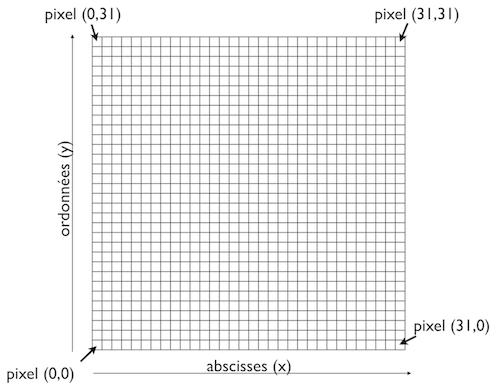
\includegraphics[width=.8\textwidth]{pixels.png}
\end{center}

\begin{exercice}
Compléter la fonction \|affichePoint| qui est utilisée
par le logiciel en mode \emph{Tracé} à chaque fois qu'il est
nécessaire de colorier un pixel.
\end{exercice}

\begin{exercice}
Compléter la fonction \|supprimePoint| qui est
utilisée par le logiciel en mode \emph{Gomme} pour effacer une zone
carrée de 3 pixels sur 3 pixels. Effacer un pixel revient à le colorier avec la couleur de fond (ici le blanc).
\end{exercice}

\begin{exercice} 
Compléter la fonction \|afficheRectangle| qui est
utilisée par le logiciel en mode \emph{Rectangle}. L'utilisateur
désigne un premier point, déplace la souris vers un deuxième point
puis relâche le bouton de la souris. Ces deux points constituent les
extrémités de la diagonale du rectangle à tracer. Le logiciel fait
alors appel à la fonction \|afficheRectangle| en donnant en
argument les coordonnées du premier point, les coordonnées du deuxième
point ainsi que la couleur demandée pour tracer les contours du
rectangle. 
\end{exercice}

\begin{exercice} 
Compléter la fonction \|remplir| qui est utilisée par
le logiciel en mode \emph{Remplir}. Les coordonnées données en
paramètres sont celles du pixel sélectionné par l'utilisateur avec son
curseur \emph{pot de peinture}. 

\begin{remarque}
  Attention, cette solution demande un peu de réflexion pour éviter de
  faire boucler la procédure de remplissage mais il existe une
  solution relativement simple et concise!
\end{remarque}

\end{exercice}

\begin{exercice} 
Compléter la fonction \|afficheLigne| qui est utilisée
par le logiciel en mode \emph{Ligne}. L'utilisateur désigne un premier
point, déplace la souris vers un deuxième point puis relâche le bouton
de la souris. Ces deux points constituent les extrémités de la ligne à
tracer. Le logiciel fait alors appel à la fonction
\|afficheLigne| en donnant en argument les coordonnées du
premier point, les coordonnées du deuxième point ainsi que la couleur
demandée pour tracer la ligne. 

\begin{remarque}
  Attention, cette fois les lignes à tracer ne sont pas forcément
  horizontales ou verticales. Comme le montre la figure ci-dessous, il
  faut savoir faire des approximations pour \emph{allumer} les pixels
  les plus proches du segment idéal.
\begin{center}
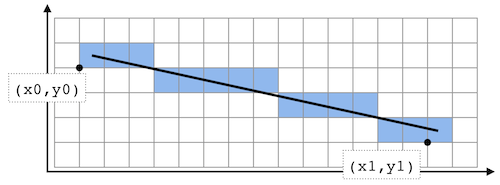
\includegraphics[width=.7\textwidth]{ligne.png}
\end{center}
\end{remarque}
\end{exercice}

\end{activite}


\end{document}

% LocalWords:  IA-IPR David Pichardie Luc proglet Javascool Démo Paintbrush
% LocalWords:  Hexa pixels pixel l'énoncé getPixel setPixel affichePoint
% LocalWords:  supprimePoint afficheRectangle afficheLigne
